%From https://egu2018.eu/PICO_how-to_guide_to_PICO.pdf
%Abstracted and templated by Brian Ballsun-Stanton, Macquarie University.
%original template by https://github.com/snowtechblog/pico-latex-presentation by Anselm Köhler

\documentclass[unknownkeysallowed,usepdftitle=false, aspectratio=169, parskip=full]{beamer}
% unknownkeysallowed is needed for mac and the newer latex version -> is more picky than before...
\usetheme[headheight=1cm,footheight=2cm]{boxes}
%\usetheme{default}


\usepackage{default}
\usepackage{graphicx}
%example pictures created via: http://lorempixel.com/1200/800/cats/Figure2/. Credit to http://lorempixel.com/images.php

\usepackage{epsfig}
\usepackage{siunitx}
\usepackage{color}
\usepackage{ifthen}
%usepackage{ragged2e}

\usepackage[T1]{fontenc}
\usepackage[utf8]{inputenc}
%https://tex.stackexchange.com/a/203804/5483

\usepackage[activate={true,nocompatibility},final,tracking=true,kerning=true,spacing=true,factor=1100,stretch=10,shrink=10]{microtype} % http://www.khirevich.com/latex/microtype/
\microtypecontext{spacing=nonfrench}

\usepackage{lipsum} % for dummy text only
\usepackage[UKenglish]{babel} %https://tex.stackexchange.com/a/27743 
\usepackage[pangram]{blindtext} % https://tex.stackexchange.com/a/48411


%\usepackage{parskip} % from https://tex.stackexchange.com/q/11622
%\setlength{\parskip}{12pt} 

%\setparsizes{\parindent}{12pt}{\parfillskip}

%\usepackage{etoolbox} % as per https://tex.stackexchange.com/a/24331
%\appto\chapterheadendvskip{\vspace{-1\parskip}}
%\setparsizes{\parindent}{50pt plus 20pt minus 30pt}{\parfillskip}

\setbeamertemplate{navigation symbols}{}%remove navigation symbols
\setbeamersize{text margin left=1cm,text margin right=1cm}

% some colors
\definecolor{grau}{gray}{.5}
\definecolor{slfcolor}{rgb}{0,0.6274,0.8353}
\definecolor{wslcolor}{rgb}{0,0.4,0.4}

% setup links
\hypersetup{%
	%linkbordercolor=green,%
	colorlinks=false,%
	pdfborderstyle={/S/U/W 0},%
	%pdfpagemode=FullScreen,%
	pdfstartpage=4%
	}

% setup some fonts
\setbeamerfont{title}{series=\bfseries, size=\small}
\setbeamerfont{author}{size*={5pt}{0pt}}
\setbeamerfont{institute}{size*={3pt}{0pt}}
\setbeamerfont{bodytext}{size=\scriptsize}
	
% Title setup	
\title{Using the Shell Command to View Multiple Text Translations}
\author{Thomas Kongonis 44618468\inst{1} (\texttt{thomas.kongonis@students.mq.edu.au})}

% add title in headbox
\setbeamertemplate{headline}
{\leavevmode
\begin{beamercolorbox}[width=1\paperwidth]{head title}
  % LOGO
  \vspace{0.1cm}
  \begin{columns}[t, totalwidth=\textwidth]
  \begin{column}[c]{1.05cm}
     
\includegraphics[width=1cm]{figure/lol.png}
  \end{column}
  % TITLE
   \begin{column}[c]{10.6cm}
   
   \centering \usebeamerfont{title} \textcolor{slfcolor}{\inserttitle} \\
   \centering \usebeamerfont{author} \color[rgb]{0,0,0} \insertauthor \\
   \vspace{-0.05cm}
   \centering \usebeamerfont{institute} \insertinstitute
  \end{column}
  % PICTURE
  \begin{column}[c]{1.15cm}
    \hspace{0.005cm}
    
\includegraphics[width=1cm]{figure/lol.png}
  \end{column}
  \end{columns}
  {\color{slfcolor}\hrule height 1pt\vspace{0.1cm}}
\end{beamercolorbox}%
}

% setup the navigation in footbox
% first set some button colors
\newcommand{\buttonactive}{\setbeamercolor{button}{bg=wslcolor,fg=white}}
\newcommand{\buttonpassive}{\setbeamercolor{button}{bg=slfcolor,fg=black}}
% now set up that the one active one gets the new color.
\newcommand{\secvariable}{nothing}
% therefore we write before each section (well, everything which should be part of the navi bar)
% the variable \secvariable to any name which is in the next function ...
\newcommand{\mysection}[1]{\renewcommand{\secvariable}{#1}
}
% ... compaired to strings in the following navibar definition ...
\newcommand{\tocbuttoncolor}[1]{%
 \ifthenelse{\equal{\secvariable}{#1}}{%
    \buttonactive}{%
    \buttonpassive}
 }
% ... here we start to set up the navibar. each entry is calling first the function \tocbuttoncolor with the argument which should be tested for beeing active. if active, then change color. afterwards the button is draw. so to change that, you need to change the argument in \toc..color, the first in \hyperlink and before each frames definition... A bit messed up, but works...
\newlength{\buttonspacingfootline}
\setlength{\buttonspacingfootline}{-0.2cm}
\setbeamertemplate{footline}
{\leavevmode
\begin{beamercolorbox}[width=1\paperwidth]{head title}
  {\color{slfcolor}\hrule height 1pt}
  \vspace{0.05cm}
  % set up the buttons in an mbox
  \centering \mbox{
    \tocbuttoncolor{abstract}
    \hyperlink{abstract}{\beamerbutton{2 Minute Madness}}
    \tocbuttoncolor{radar}
    \hspace{\buttonspacingfootline}
      \hyperlink{radar}{\beamerbutton{The Text}}

    \tocbuttoncolor{line}
    \hspace{\buttonspacingfootline}
      \hyperlink{line}{\beamerbutton{The Unix Shell}}
    \tocbuttoncolor{major}
    \hspace{\buttonspacingfootline}
      \hyperlink{major}{\beamerbutton{Example}}
    \tocbuttoncolor{slab}
    \hspace{\buttonspacingfootline}
      \hyperlink{slab}{\beamerbutton{Template}}
    \tocbuttoncolor{minor}
    \hspace{\buttonspacingfootline}
      \hyperlink{minor}{\beamerbutton{Conclusion}}
    \tocbuttoncolor{conclusion}
    
    % this last one should normaly not be used... it will open the preferences to change the 
    % behaviour of the acrobat reader in fullscreen -> usefull in pico...
    \setbeamercolor{button}{bg=white,fg=black}
    % for presentation
    %\hspace{-0.1cm}\Acrobatmenu{FullScreenPrefs}{\beamerbutton{\#}}
    % for upload
    
     
\Acrobatmenu{FullScreenPrefs}{\vspace{0.3cm}\hspace{0.24cm}\mbox{%
      
\includegraphics[height=0.04\textheight,keepaspectratio]{%
	  figure/CreativeCommons_Attribution_License.eps}%
	  }}
   }
    \vspace{0.05cm}
\end{beamercolorbox}%
}


\begin{document}


%%%%%%%%%%%%%%%%%%%%%%%%%%%%%%%%%%%%%%%%%%%%%%%%%%%%%%%%%%%%%%%%%%%%%%%%%%
\mysection{abstract}
%%%%%%%%%%%%%%%%%%%%%%%%%%%%%%%%%%%%%%%%%%%%%%%%%%%%%%%%%%%%%%%%%%%%%%%%%%
\begin{frame}\label{\secvariable}

\usebeamerfont{bodytext}


\parbox{\linewidth}{


\vspace{12pt}

Background: Dealing with Philosophical texts is confusing enough! Add a different language into the mix and there is almost a guarantee that something will be lost in translation. What is the remedy to this? Multiple Translations of course!

 \vspace{12pt}
 
Aims/Objectives: The aim was to be able to utilise the Unix Shell to be able to run an easy script to pull 5 iterations of a single translated word and show them up consecutively on the console. 

 \vspace{12pt}
 
Outcome: The outcome wasn't as glamorous, after returning to the drawing board and experimenting, creating a directory and shell scripts to pull translated chapters and consecutively displaying them was the compromise i completed.  
}


   
\end{frame}

\begin{frame}\label{\secvariable}
  \begin{columns}[t]
  %https://tex.stackexchange.com/a/7452/5483
  \begin{column}[c]{0.45\textwidth}
%http://lorempixel.com/1200/800/cats/Figure2/     
%http://lorempixel.com/1200/800/cats/Figure3/
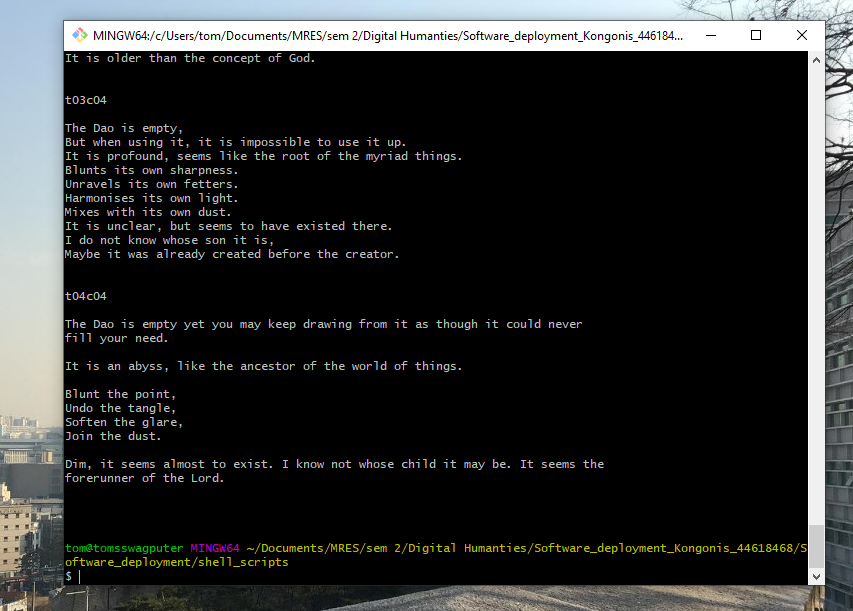
\includegraphics[width=1\textwidth,height=0.5\textheight,keepaspectratio]{%
figure/Example02.png}\\
\vspace{12pt}
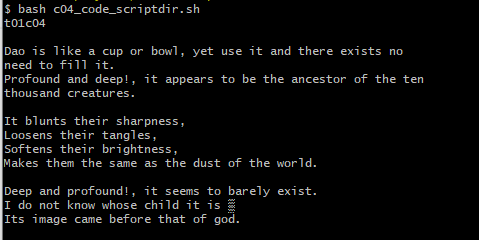
\includegraphics[width=1\textwidth,height=0.5\textheight,keepaspectratio]{%
figure/Untitled5.png}
    \end{column}
    \begin{column}[c]{0.45\textwidth}
    \parbox{\linewidth}{

      Significance: This tool provides low stress on the computer and no extra word documents, browsers or pdfs need to be loaded. Whilst you're working away if you need to see extra translations open up your shell and autofill the code and there you go! This makes the process of referring to multiple translations significantly easier. 
      
      \vspace{12pt}
      
     Example: The Image to the left shows an example of the script being utilised from the shell. As you can see two of the chapters are in the window. (Project Gutenburg 2015)
      }
    \end{column}
    
  \end{columns}

  
\end{frame}

%%%%%%%%%%%%%%%%%%%%%%%%%%%%%%%%%%%%%%%%%%%%%%%%%%%%%%%%%%%%%%%%%%%%%%%%%%
\mysection{radar}
%%%%%%%%%%%%%%%%%%%%%%%%%%%%%%%%%%%%%%%%%%%%%%%%%%%%%%%%%%%%%%%%%%%%%%%%%%
\begin{frame}\label{\secvariable}
  \begin{columns}[t]
  %https://tex.stackexchange.com/a/7452/5483
    \begin{column}[c]{0.45\textwidth}
    \parbox{\linewidth}{

   Dao De Jing: This text is an ancient Chinese Philosophical text dating back thousands of years to a mysterious author named Laozi. It can be traced as far as 2500 years to a set of ancient bamboo scripts called the Guodian Wuxing. (Csikszentmihayli 2004)
      
      \vspace{12pt}
      
	  The text is quite confusing and there are many translations, most of which are public domain or fair use. 
     
     \vspace{2mm}
     Image:
      
  \texttt{https://languechinoise.wordpress.com/}   

            }
    \end{column}
    \begin{column}[c]{0.45\textwidth}
%http://lorempixel.com/1200/800/cats/Figure2/     
%http://lorempixel.com/1200/800/cats/Figure3/
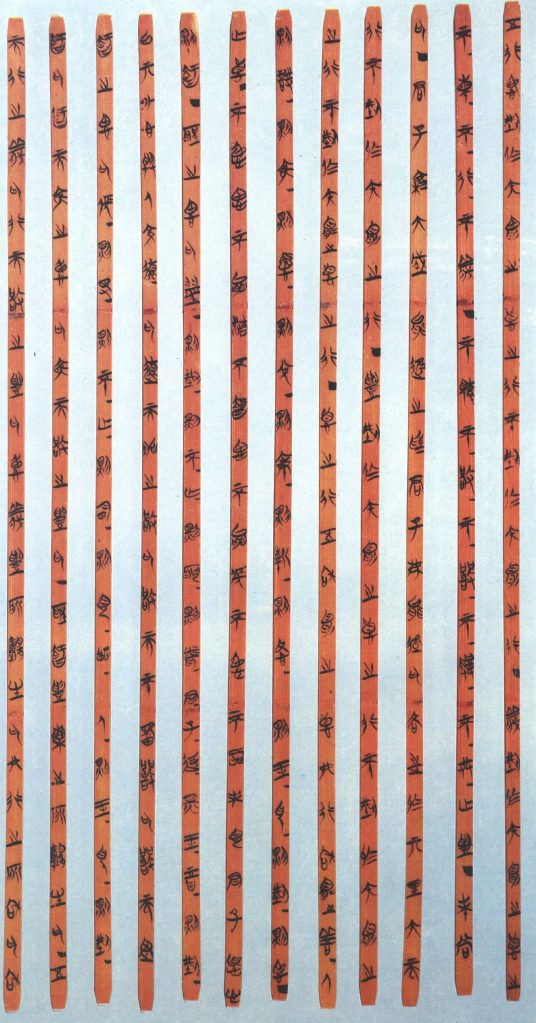
\includegraphics[width=2\textwidth,height=1\textheight,keepaspectratio]{%
figure/p0010.png}\\
\vspace{12pt}

    \end{column}
  \end{columns}

  
\end{frame}

%%%%%%%%%%%%%%%%%%%%%%%%%%%%%%%%%%%%%%%%%%%%%%%%%%%%%%%%%%%%%%%%%%%%%%%%%%
\mysection{line}
%%%%%%%%%%%%%%%%%%%%%%%%%%%%%%%%%%%%%%%%%%%%%%%%%%%%%%%%%%%%%%%%%%%%%%%%%%
\begin{frame}\label{\secvariable}
\begin{center}
  \vspace{-0.5cm}
  %http://lorempixel.com/1200/800/cats/Figure4/
 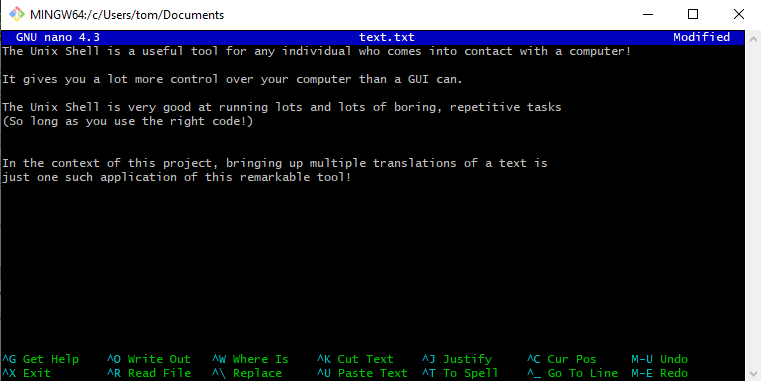
\includegraphics[width=1.20\textwidth,height=0.95\textheight,keepaspectratio]{%
  figure/eg55.png}
\end{center}
  \vspace{-0.5cm}
  
  
\end{frame}

%%%%%%%%%%%%%%%%%%%%%%%%%%%%%%%%%%%%%%%%%%%%%%%%%%%%%%%%%%%%%%%%%%%%%%%%%%
\mysection{major}
%%%%%%%%%%%%%%%%%%%%%%%%%%%%%%%%%%%%%%%%%%%%%%%%%%%%%%%%%%%%%%%%%%%%%%%%%%
\begin{frame}\label{\secvariable} %%Eine Folie
\begin{center}
%http://lorempixel.com/1200/800/cats/Figure5/
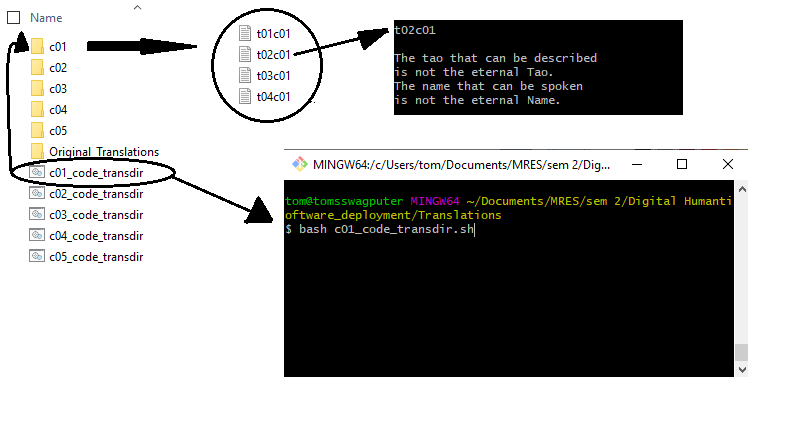
\includegraphics[width=1.05\textwidth,height=0.85\textheight,keepaspectratio]{%
figure/eg22.png}
\end{center}
This is an simple example of the script in action
\end{frame}

%%%%%%%%%%%%%%%%%%%%%%%%%%%%%%%%%%%%%%%%%%%%%%%%%%%%%%%%%%%%%%%%%%%%%%%%%%
\mysection{slab}
%%%%%%%%%%%%%%%%%%%%%%%%%%%%%%%%%%%%%%%%%%%%%%%%%%%%%%%%%%%%%%%%%%%%%%%%%%
\begin{frame}\label{\secvariable}
%http://lorempixel.com/1200/800/cats/Figure6/

   \begin{flushleft}
   \parbox{\linewidth}{
\begin{itemize}
\item{Template: I have created a template directory so that anyone can replicate this with other translations. This includes scripts for correct document names and creation also.} 
\end{itemize}
}
\begin{flushright}
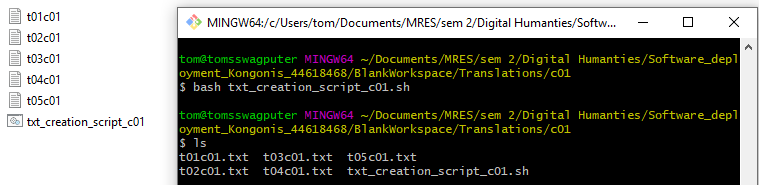
\includegraphics[width=1.7\textwidth,height=0.50\textheight,keepaspectratio]{%
figure/eg444.png}
\end{flushright}
\end{flushleft}
\end{frame}








%%%%%%%%%%%%%%%%%%%%%%%%%%%%%%%%%%%%%%%%%%%%%%%%%%%%%%%%%%%%%%%%%%%%%%%%%%
\mysection{minor}
%%%%%%%%%%%%%%%%%%%%%%%%%%%%%%%%%%%%%%%%%%%%%%%%%%%%%%%%%%%%%%%%%%%%%%%%%%


%%%%%%%%%%%%%%%%%%%%%%%%%%%%%%%%%%%%%%%%%%%%%%%%%%%%%%%%%%%%%%%%%%%%%%%%%%

%%%%%%%%%%%%%%%%%%%%%%%%%%%%%%%%%%%%%%%%%%%%%%%%%%%%%%%%%%%%%%%%%%%%%%%%%%
\begin{frame}\label{\secvariable}

%

Location of Proof of Concept and Template: \url{https://github.com/MQ-FOAR705/Tom_Kongonis_44618468_POC.git}

\vspace{5mm}

\begin{itemize}
\item{\textbf{Bibliography:}}
\item{Csikszentmihalyi, M., 2004. Material Virtue Ethics and the Body in Early China. 1st ed. Leiden: Brill NV.}

\item{Tzu, L., 2015. Dao De Jing. 1st ed. s.l.:Project Gutenberg.}
\item{All images except for the Wuxing script one (Which was refrenced) were made by me.}
\end{itemize}

\end{frame}

%%%%%%%%%%%%%%%%%%%%%%%%%%%%%%%%%%%%%%%%%%%%%%%%%%%%%%%%%%%%%%%%%%%%%%%%%%
\mysection{conclusion}
%%%%%%%%%%%%%%%%%%%%%%%%%%%%%%%%%%%%%%%%%%%%%%%%%%%%%%%%%%%%%%%%%%%%%%%%%%



\end{document}
